\section{\sys}
\label{s:method}
\begin{figure}[t]
    \centering
    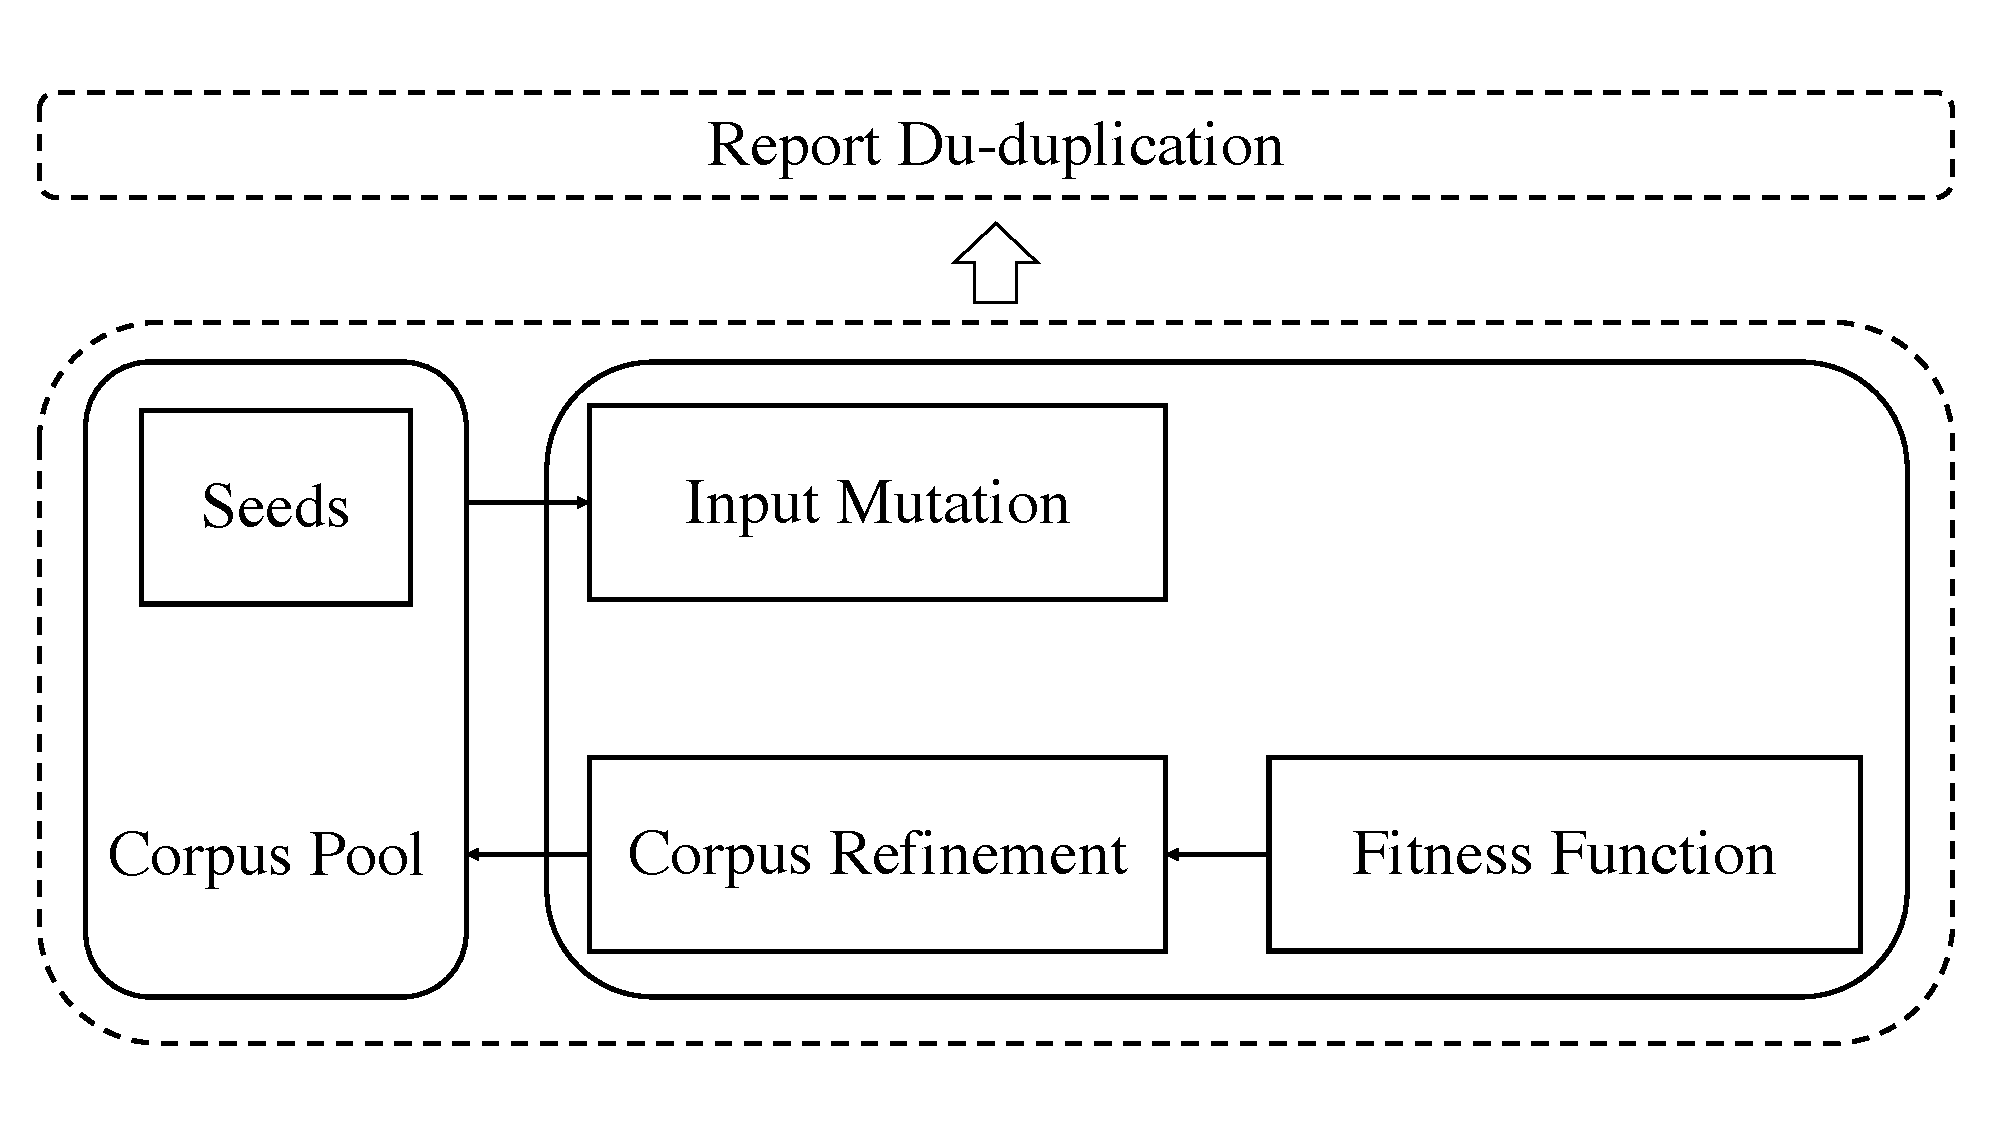
\includegraphics[width=0.45\textwidth]{fig/netfuzz.pdf}
    \caption{The architecture of \sys.
    }
    \label{fig:arch}
\end{figure}

Though we have characterized known performance bugs, %in \autoref{s:study},
%
it is unclear if there exist many unknown performance bugs in the network operating systems.
%
Therefore, we try to detect performance bugs in real-world network operating systems.
%
We focus on CPU resource exhaustion performance bugs in this work because they are the dominant type of performance bugs.
%Due to the high false positives and the excessive manual efforts required in static analysis \cite{rathnayake2014static, wustholz2017static},
%
%dynamic methods are usually preferred.
%

To avoid the high false-positive rates in static analyses \cite{nistor2013toddler,nistor2015caramel},
%
we propose to use dynamic fuzz testing to detect and exploit performance bugs.
%aiming to eliminate the false-positive reports.
%
%Similar to existing works in ReDoS \cite{freezing},
%we also leverage a black-box dynamic testing method to detect performance bugs.
%
%
%The main idea behind our methodology is to leverage test cases to dynamically test real-world applications and platforms and check whether they are vulnerable to performance bugs.
%
To do so, we face a technical challenge.
%
Since many distinct inputs can trigger the same performance bug, it is naturally challenging to accurately de-duplicate the bug reports.
%
Prior performance bug fuzzers \cite{slowfuzz, hotfuzz} do not try to de-duplicate performance bugs.
%
Other fuzzers for detecting \emph{memory corruptions} de-duplicate bugs using the unique memory footprints (\eg{,} coverage profiles and call stacks \cite{klees2018evaluating}) when the bugs are triggered,
%
whereas one \emph{performance bug} can potentially exhibit different memory footprints.
%distinguish abnormal program behaviors from normal ones.
%
%Third, diverse implementations in different programming languages make the bug detection task even harder.
%
%Developing a language-agnostic solution is hard.

%\subsection{Overview}
We overcome these challenges with \sys.
%
The overall methodology is depicted in \autoref{fig:arch}.
%
\sys follows the general fuzzing workflow and is built on top of AFL \cite{afl}.
%
Inside the main fuzzing loop, 
%
to guide the fuzzer to detect CPU resource exhaustion performance bugs,
we use a fitness function to measure if an input should be favored or not
%
(\autoref{s:method-fitness-function}).
%
The fitness function considers both code coverage and resource usage.
%
To report only unique bugs, we transform the execution trace of each report into a vector.
%
We compute the cosine similarity of vector (report) pairs and group highly similar reports as duplicate ones (\autoref{s:method-de-duplicating}).
%
We then present the implementation details (\autoref{s:method-impl}).

\subsection{Fitness Function and Performance Bug Detection}
\label{s:method-fitness-function}
\sys uses a fitness function to decide whether to favor a test case or not.
%
%Coverage-based fitness function enables the fuzzers to explore more new code locations.
%
%
We include both the coverage and the control flow graph (CFG) edge hits into the fitness function.
%
As in other works \cite{oss-fuzz, peng2018tfuzz, klees2018evaluating}, the coverage feedback drives \sys to explore more newly discovered code.
%
Only it, however, is not sufficient for our purpose as it does not consider loop iterations which are crucial for detecting high-complexity performance bugs \cite{slowfuzz}.
%
The CFG edge hits, standing for the times a CFG edge is visited under a test case, enables \sys to explore \emph{computationally expensive} paths.
%
As stated in prior work \cite{perffuzz}, many programs (\eg{,} PHP hash functions \cite{perffuzz, php-hash}) do have non-convex performance space.
%
We thus do not use the execution path length (\eg{,} number of executed instructions) to guide \sys because it might fail to find the performance issues caused by local maxima.
%to the ability to overcome local maxima in a non-convex performance space
%
Therefore, as in the state-of-the-art work, PerfFuzz \cite{perffuzz}, we design \sys to favor those test cases that maximize certain CFG edge hits to better detect performance bugs.
%
In this way, \sys tends to select test cases to either trigger new code or exhaust certain CFG edges.
%
Note that we do not use runtime CPU usage or concrete execution time as the metric,
%
because they show large variations affected by many uncontrollable factors, such as fuzzer's concurrent features and the characteristics of testing applications.

\iffalse
%With the fitness function, \sys favors several cases that maximize at least one CFG edge during fuzzing.
As stated in \cite{hotfuzz}, an explicit definition of performance bugs of a testing program relies on domain knowledge and manual analysis.
%
This is realistic and pragmatic because it is necessary to understand intended resource consumption bounds.
%
%Not all these test cases necessarily trigger performance bugs as their overall performance slowdown might be light.
%
%
Therefore,
%
we evaluate the test cases to obtain their execution path lengths.
%
We configure a resource computation threshold and label those cases that exceed it as performance bugs.
\fi
%
%

We design a statistical model to accurately identify performance bugs.
Our statistical model first obtains the normal program execution behaviors to label abnormal ones as performance bugs.
%
In particular, though the fitness function favors the local maxima, we still consider the total execution path length as the criteria of performance bugs.
%
The execution path length is calculated as the sum of the CFG edge hits under a test case.
%
We first prepare abundant random normal test cases;
%
we feed each test case to the testing program and obtain the corresponding execution path length.
%
We calculate the the mean ($l_{\mu}$) and the standard deviation ($l_{\sigma}$) of the execution path lengths ($l_i$).
%
We label a case as a performance bug if its execution path exceeds the normal level to a certain extent.
%
%as in Rampart \cite{rampart}, a defense against sophisticated CPU-exhaustion DoS attacks,
%
According to Chebyshev inequality (as shown in \autoref{chebyshev}),
%can measure the probability that one observation differs from the mean of the samples.
%
the probability of the random variable $l_{i}$ that is k-standard deviations away from the mean ($l_{\mu}$) is no more than ${1}/{k^2}$.
%
%Even though we enforce that all test cases are in the size of $m$, we do not assume any underlying distributions of the random variable $T_{r}$ on the uses of Chebyshev inequality.
Since only in rare cases would the execution path length significantly deviate from the normal situations,
%
therefore, we label a performance bug if its execution path length $l_{t}$ is more than $kl_{\sigma}$ away from the $l_{\mu}$ (see \autoref{label}).
%
%
%
%We configure a maximum threshold for a high detection efficiency because some attack inputs may take several hours to process.

\begin{equation} \label{chebyshev}
    P(|l_{i}-l_{\mu}| > k l_{\sigma}) \leq \frac{1}{k^2}
\end{equation}

\begin{equation} \label{label}
    l_{t} > l_{\mu} + kl_{\sigma}
\end{equation}

\subsection{Report De-Duplication}
\label{s:method-de-duplicating}

Though different test cases could all exceed the threshold, they could actually trigger the same performance bug.
%
De-duplicating the bug reports is necessary for a more precise result,
whereas prior works \cite{slowfuzz, perffuzz} do not apply automated methods to de-duplicate the reports.
%
Existing fuzzing works identify unique bugs using the call stack for memory corruptions (\eg{,} crashes).
%
However, it does not fit well our purposes for performance bug de-duplication.
%
Though we can possibly collect the call stack as well (\eg{,} by forcibly terminating the program at some point), the call stack might not be accurate enough to differentiate unique bugs.
%
This is because the exactly critical call stack for a performance bug can hardly be accurately exposed.
%
Unlike memory corruptions that have a deterministic call stack when a bug is triggered,
performance bugs might exhibit diverse call stacks depending on when to obtain them.
%
Therefore, a better report de-duplication method is needed.

We propose a new bug de-duplicating approach by merging reports with similar execution traces.
%
The high-level idea is that different exploiting inputs of the same performance bug should exhibit similar execution traces, \ie{,} most CFG edges are visited in similar frequencies.
%
In particular, we apply the test cases in the reports to the instrumented target software and obtain the CFG edge hits for each edge.
%
We summarize the unique CFG edges that are visited in all reports during fuzz testing into an $n$-dimensional vector space, where $n$ is the total number of unique CFG edges being visited and each dimension in the vector space corresponds to a CFG edge.
%
For each report, we construct an edge-hit vector, \eg{,} $\vv{v}=\left (c_1, c_2, ... , c_n \right )$.
%
Each dimension ($c_i$) represents the hit count of the $i$th CFG edge in that report.
%is the CFG edge hits, which is a non-negative value, \ie{,} $c_i \geq 0$.
%
%$c_i$ is 0 only when the corresponding CFG edge is not visited in the execution trace of the report.
%
To consider if two reports point to the same bug, we construct their edge-hit vectors (\eg{,} $\vv{v}, \vv{v}'$) and compute the cosine similarity (as shown in \autoref{sim}).
%\WM{Do two vectors always have the same number of unique edges? How do you order the edges in the vector?}
%
Cosine similarity is based on the inner product of the two vectors and thus naturally assigns higher weights to the dimensions with larger values (\ie{,} edges visited most).
%
%When triggering a performance bug, certain CFG edges are usually visited more than the others \ie{,} hot edges.
%
Therefore, we calculate the cosine similarity between every two reports and merge reports as the same bug if the cosine similarity of their corresponding edge-hit vectors exceeds a threshold.
%
%We believe it can accurately measure the similarity of the two reports.

\begin{equation} \label{sim}
    Sim(\vv{v}, \vv{v}') = \frac{\vv{v}\cdot \vv{v}'}{|\vv{v}||\vv{v}'|}\
    = \frac{\sum_{j=1}^{n}{c_jc_j'}}{\sqrt{\sum_{j=1}^{n}{c_j^2}} \sqrt{\sum_{j=1}^{n}{c_j'^2}} }
\end{equation}

%
\iffalse
We take a two-step matching approach to efficiently de-duplicate reports.
%
%the simplest algorithm is to compute the cosine similarity of every two reports.
%a program usually contains over 10K distinct CFG edges thus the vector space has over 10K dimensions correspondingly;
%Since
%
%The time complexity of calculating the cosine complexity of two $n$-demensional vectors is roughly $O(n)$ as each dimension is computed for a constant time.
%
%Therefore, the time complexity of the simple algorithm is $O(n \cdot m^2)$, where $m$ is the total number of reports.
%
%However,
%it is very expensive to perform cosine similarity calculation for such an algorithm time complexity because the edge vector space usually has large dimensions (\ie{,} $m >> n$).
%
%
%fuzzing usually produces about 1K reports.
%
%
%\WM{The description was not that clear.}
%\WM{You reduce the vector size like you downsample images, from 100 dimensions into 10 dimensions of which each one is the average value of the previously adjacent 10 dimensions. Then you still do a pair-wise comparison but it would be much more efficient. Then the similar ones are grouped into a cluster.}
First, 
since the edge vector space is usually large, \eg{,} $n > 10,000$,
we reduce the size of the edge vector space by merging a few (\eg{,} 100) adjacent dimensions into one dimension taking their average value.
%
The reduced vector serves as a rough signature of a report.
%
We then compute the cosine similarity of every two reduced vectors and group similar reports into buckets in a coarse-grained manner.
%
%Note that this is more efficient than calculating the exact cosine similarity of original vectors as the vector space size is hugely reduced.
%
%Specifically, we use a relatively lower threshold to cluster the reports into several buckets.
%
Second, within each bucket of similar reports, we compute the exact cosine similarity between two original vectors (reports), classify highly similar ones as a distinct bug.
%
In this way, compared to calculating the exact cosine similarity between every two reports, the time complexity can potentially be reduced by several orders of magnitude.
%
%We will discuss the threshold $sim_t$ later in \autoref{s:eval-parameter}
%
%We configure a maximum threshold for a high detection efficiency because some attack inputs may take several hours to process.
\fi

%

\subsection{Implementation}
\label{s:method-impl}
We implemented the fuzzing part of \sys above an AFL-based fuzzer, PerfFuzz \cite{perffuzz}.
%
Specifically,
we enhanced a C/C++ compiler to instrument the testing software;
we modified AFL's \cc{showmap} functionality to trace the execution on the instrumented applications to obtain the CFG edge hits for report de-duplication.
%
%We implemented our report de-duplicating part with 500 lines of Python code.



\iffalse
\subsection{Performance Bug Detection}
\label{s:method-model}
We build a statistical model to accurately distinguish the normal behaviors and abnormal ones for detecting performance bugs.
%
%\ZMX{A statistical model for what?}
%
As discussed before, using execution time is a common practice in identifying performance bugs \cite{rampart, freezing},
%\ZMX{Exeuction time is not a practice.}
%
so we also use it in our statistical model.
%
%
Our statistical model requires a training stage by feeding the program with $N_r$ random test cases ($I_{r}$) and obtaining the corresponding execution time ($T_{r}$).
%
To eliminate the impacts of the input sizes,
%
we require all the test cases used in our statistical model to be in a constant size, $m$.
%
%Based on basic statistic analysis,
%Statistically, we can regard the execution time as a random variable.
%\ZMX{$T_{r}$ is the set of execution time on a set of test cases. Why can it be a random ``variable''?}
%
We compute the mean ($T_{\mu}$) and the standard deviation ($T_{\sigma}$) of the $N_r$ execution times ($T_{r}$),
%
%Thus its probability distribution can roughly belong to normal distributions.

Our statistical model requires a training stage by feeding the program with $N_r$ random test cases ($I_{r}$) and obtaining the corresponding execution time ($T_{r}$).
%
To eliminate the impacts of the input sizes,
%
we require all the test cases used in our statistical model to be in a constant size, $m$.
%
%Based on basic statistic analysis,
%Statistically, we can regard the execution time as a random variable.
%\ZMX{$T_{r}$ is the set of execution time on a set of test cases. Why can it be a random ``variable''?}
%
We compute the mean ($T_{\mu}$) and the standard deviation ($T_{\sigma}$) of the $N_r$ execution times ($T_{r}$),
To identify performance bugs that could cause spend the underlying network operating systems an extremely long execution time,
%
%as in Rampart \cite{rampart}, a defense against sophisticated CPU-exhaustion DoS attacks,
%
as in \cite{rampart}, we also use the Chebyshev inequality (as shown in \autoref{equ1}) to measure the probability that one observation differs from the mean of the samples.
%
Specifically, the probability of the random variable $T_{r}$ that is k-standard deviations away from the mean ($T_{\mu}$) is no more than ${1}/{k^2}$.
%
Even though we enforce that all test cases are in the size of $m$, we do not assume any underlying distributions of the random variable $T_{r}$ on the uses of Chebyshev inequality.
%
Therefore, in the testing stage, we use \autoref{equ2} to label a performance bug if its execution time on a test case $T_{test}$ is more than $kT_{\sigma}$ away from the mean ($T_{\mu}$) or reaches the maximum time threshold ($T_{max}$).
%
We configure a maximum threshold for a high detection efficiency because some attack inputs may take several hours to process.

\begin{equation} \label{equ1}
    P(|T_{r}-T_{\mu}| > kT_{\sigma}) \leq \frac{1}{k^2}
\end{equation}

\begin{equation} \label{equ2}
    T_{test} > min(T_{\mu} + kT_{\sigma}, T_{max})
\end{equation}
\fi
